\documentclass{article}

\usepackage{ragged2e}
\usepackage{graphicx}
\usepackage{amsmath}

\begin{document}

\begin{flushright}
    \noindent
    Rodrigo Becerril Ferreyra\\
    CECS 211 Section 01\\
    2019-09-04
\end{flushright}

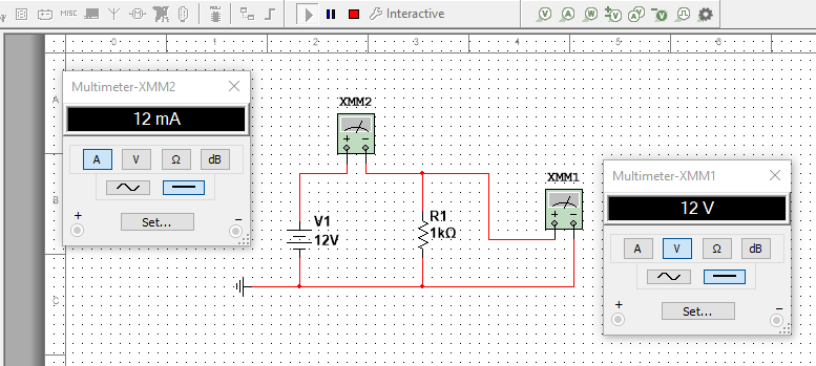
\includegraphics[width=\textwidth]{Lab1.png}
\\
\\
\\
\\
\indent
XMM1: The voltage on the multimeter (which is set on voltage
mode) reads 12~V.
This is because the DC power supply is supplying 
12~V to the wire.

XMM2: This multimeter is set to read current in Amperes. Without
looking at the multimeter, we can calculate the expected
value for current using Ohm's Law:
\begin{align*}
    V &=IR \\
    1\text{ V} &= 1\text{ A} \times 1\text{ }\Omega
\end{align*}

In this case, we have 12~V and 1k~$\Omega$:

\begin{align*}
    12\text{ V} &= \text{? A} \times 1\text{ k}\Omega \\
    \frac{12\text{ V}}{1 \times 10^3 \Omega} &= \text{? A} \\
    \text {? A} &= 12 \times 10^{-3}\text{ A} = 12\text{ mA}
\end{align*}

Sure enough, the multimeter XMM2 reads 12~mA.

\end{document}